\subsection{Dependencies}

The following table contains dependencies in the backend application and the date of their addition to the project. The topic of dependencies is also introduced in the Licenses section, where we have collected all the dependencies with their licenses by several tools. Those files can also be found on the GitHub repository\cite{githubrepo}.

\newpage
\begin{table}[h!]
\centering
    \scalebox{0.9}{
        \begin{tabular}{ p{0.45\linewidth} p{0.35\linewidth} r p{0.05\linewidth} }
          \toprule
          Dependency & \multicolumn{1}{c}{Description} & \multicolumn{1}{c}{Date of Addition} \\
          
          \midrule
          \addlinespace[0.2cm]
          
          \textbf{dotnet / aspnetcore} & .NET framework for building cross-platform applications & 02.18. \\
          
          \addlinespace[0.2cm]
          \midrule
          \addlinespace[0.2cm]
          
          \textbf{dotnet / efcore} & Object-database mapper for .NET & \\
          
          \addlinespace[0.2cm]
          
          \textbf{\small Microsoft.EntityFrameworkCore.Design} & Design-time logic for Entity Framework Core, used for migrations & 03.11. \\
          
          \addlinespace[0.2cm]
          
          \textbf{\small Microsoft.EntityFrameworkCore.InMemory} & In-memory database provider for Entity Framework Core & 03.30. \\
          
          \addlinespace[0.2cm]
          
          \textbf{\small Microsoft.EntityFrameworkCore.Sqlite} & SQLite database provider for Entity Framework Core & 02.08. \\
          
          \addlinespace[0.2cm]
          \midrule
          \addlinespace[0.2cm]
          
          \textbf{JamesNK / Newtonsoft.Json} & JSON framework for .NET & 02.18. \\
          
          \addlinespace[0.2cm]
          \midrule
          \addlinespace[0.2cm]
          
          \textbf{\small PomeloFoundation/ Pomelo.EntityFrameworkCore.MySql} & MySQL database provider for Entity Framework Core & 03.11. \\
          
          \addlinespace[0.2cm]
          \midrule
          \addlinespace[0.2cm]
          
          \textbf{prometheus-net} & Library to instrument metrics with code & 03.05. \\
          
          \addlinespace[0.2cm]
          \midrule
          \addlinespace[0.2cm]
          
          \textbf{\small Daniel15 / prometheus-net.SystemMetrics} & Exporting essential metrics to Prometheus & 03.20. \\
          
          \addlinespace[0.2cm]
          \midrule
          \addlinespace[0.2cm]
          
          \textbf{saleem-mirza / serilog-enrichers-context} & Enriching logging with custom properties & 03.24. \\
          
          \addlinespace[0.2cm]
          \midrule
          \addlinespace[0.2cm]
          
          \textbf{serilog} & Logging framework for .NET \\
          
          \addlinespace[0.2cm]
          
          \textbf{serilog-enrichers-environment} & Enriching logging with information of process environment & 03.24. \\
          
          \addlinespace
          
          \textbf{serilog-extensions-hosting} & Routes log messages to sinks & 03.05. \\
          
          \addlinespace
          
          \textbf{serilog-sinks-console} & Writing logs to standard output & 03.05. \\
          
          \addlinespace
          
          \textbf{serilog-sinks-file} & Writing logs to files & 03.06. \\
          
          \addlinespace[0.2cm]
          \midrule
          \addlinespace[0.2cm]
          
          \textbf{DataDog / serilog-sinks-datadog-logs} & Sink that sends log events to DataDog & 03.24. \\
          
          \addlinespace[0.2cm]
          \midrule
          \addlinespace[0.2cm]
          
          \textbf{shakenetwork / sonaranalyzer-dotnet} & Analyzers for C\# & 03.20. \\
          
          \addlinespace[0.2cm]
          \midrule
          \addlinespace[0.2cm]
          
          \textbf{coverlet-coverage / coverlet.collector} & Code coverage for .NET & 02.12. \\
          
          \addlinespace[0.2cm]
          \midrule
          \addlinespace[0.2cm]
          
          \textbf{fluentassertions / fluentassertions} & Extensions to specify expected outcome of tests & 03.18. \\
          
          \addlinespace[0.2cm]
          \midrule
          \addlinespace[0.2cm]
          
          \textbf{microsoft / vstest} & Test platform for running tests and collect diagnostics & 02.12. \\
          
          \addlinespace[0.2cm]
          \midrule
          \addlinespace[0.2cm]
          
          \textbf{moq / Moq.AutoMocker} & Building instances for unit testing & 03.18. \\
          
          \addlinespace[0.2cm]
          \midrule
          \addlinespace[0.2cm]
          
          \textbf{nunit} & Unit Testing framework for .NET \\
          
          \addlinespace[0.2cm]
          
          \textbf{nunit3-vs-adapter} & Test adapter for running unit tests & 02.12. \\
          
          \bottomrule
        \end{tabular}
    }
    
    \caption{Back-end Dependencies}
    \label{fig:backendDependencyTable}
\end{table}

{\color{red} \textbf{At this point in time I have yet to find a reliable tool that creates a graph for nuget packages}}

The following table contains dependencies in the frontend application and the date of addition to the project:

\begin{table}[h!]
\centering
    \begin{tabular}{ p{0.45\linewidth} p{0.35\linewidth} r p{0.05\linewidth} }
      \toprule
      Dependency & \multicolumn{1}{c}{Description} & \multicolumn{1}{c}{Date of Addition} \\
      
      \midrule
      \addlinespace[0.2cm]
      
      \textbf{vuejs / core} & JavaScript framework for building UIs & 02.10. \\
      
      \addlinespace[0.2cm]
      \midrule
      \addlinespace[0.2cm]
      
      \textbf{vuejs / cli} & Extensible tooling built on top of webpack for the Vue ecosystem & \\
      
      \addlinespace[0.2cm]
      
      \textbf{cli-plugin-babel} & Convert code into backwards compatible versions of JavaScript & 02.10. \\
      
      \addlinespace[0.2cm]
      
      \textbf{cli-plugin-router} & Plugin for router to make SPAs & 02.10. \\
      
      \addlinespace[0.2cm]
      
      \textbf{cli-plugin-vuex} & State management library & 02.10. \\
      
      \addlinespace[0.2cm]
      
      \textbf{cli-service} & Scaffolding new projects, Vue commands in terminal & 02.10. \\
      
      \addlinespace[0.2cm]
      
      \textbf{compiler-sfc} & Part of main vue package, contains lower level utilities & 02.10. \\
      
      \addlinespace[0.2cm]
      \midrule
      \addlinespace[0.2cm]
      
      \textbf{axios} & HTTP client & 02.10. \\
      
      \addlinespace[0.2cm]
      \midrule
      \addlinespace[0.2cm]
      
      \textbf{zloirock / core-js} & JS library for language and browser-specific extensions & 02.10. \\
      
      \addlinespace[0.2cm]
      \midrule
      \addlinespace[0.2cm]
      
      \textbf{motdotla / dotenv} & Loading .env variables & 02.13. \\
      
      \addlinespace[0.2cm]
      \midrule
      \addlinespace[0.2cm]
      
      \textbf{sass / dart-sass} & CSS preprocessor to generate CSS from unique syntax & 02.10. \\
      
      \addlinespace[0.2cm]
      \midrule
      \addlinespace[0.2cm]
      
      \textbf{webpack-contrib / sass-loader} & To compile SASS to CSS & 02.11. \\
      
      \addlinespace[0.2cm]
      \midrule
      \addlinespace[0.2cm]
      
      \textbf{epicmaxco / vuestic-ui} & UI library for Vue3 & 02.11. \\
      
      \bottomrule
    \end{tabular}
    
    \caption{Front-end Dependencies}
    \label{fig:frontendDependencyTable}
\end{table}

The visualization of all the dependencies has been made by an online tool~\cite{packageLockVisualizer} and it has produced the following graph~\cite{frontendDependencyGraph}:

% 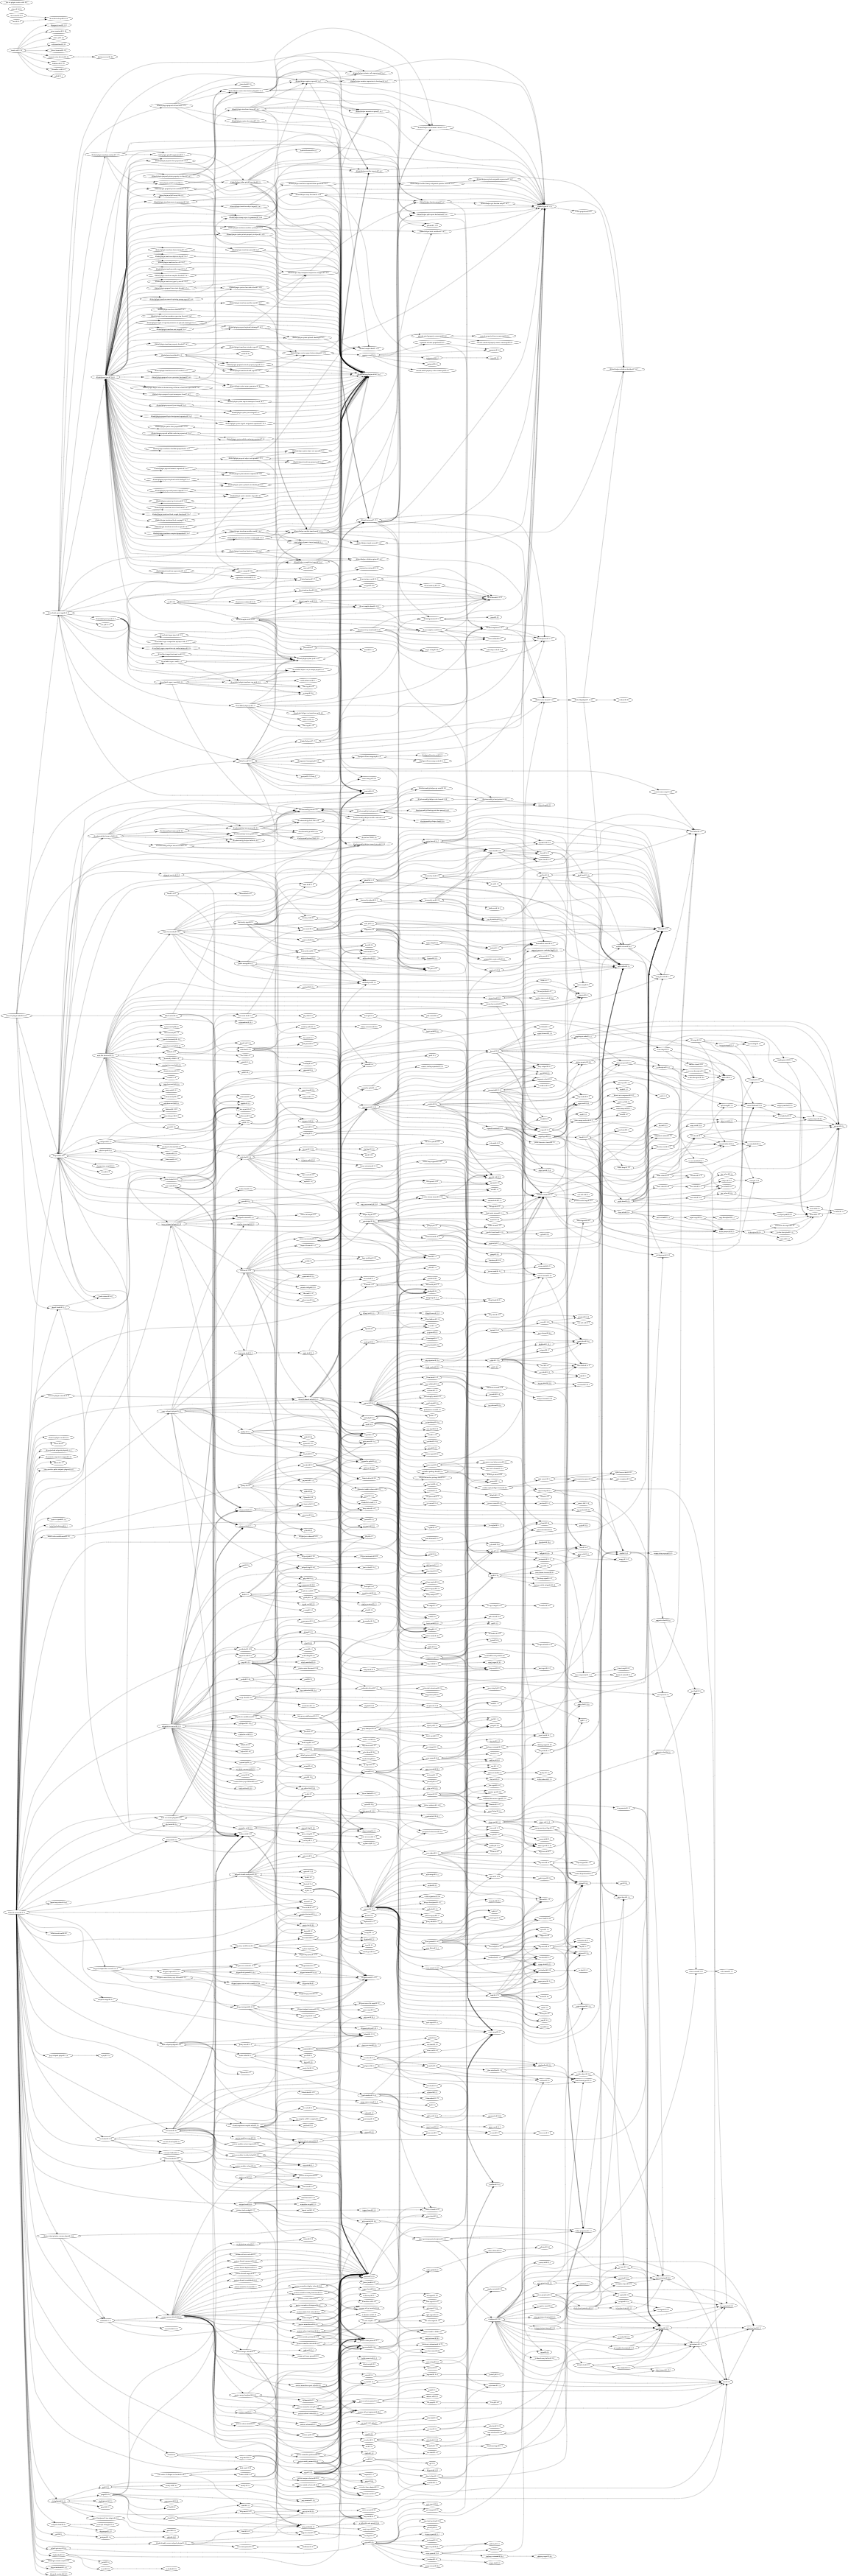
\includegraphics[scale=0.05]{images/dependency_graphs/minitwit_fe_package_lock_graph.png}
